%%%%% Úvod
%%%%% ------------------------------------------------------------
\chapter*{Úvod}
\addcontentsline{toc}{chapter}{Úvod}

%%% Sekce - Prodej vstupenek
%%%%% Wording: ✅
%%%%% Styling: ✅
%%%%% References: ✅
%%%%% Grammar: ✅
%%% --------------------------------------------------------------
\section*{Prodej vstupenek}
\addcontentsline{toc}{section}{Prodej vstupenek}
\label{sec:uvod-prodej-vstupenek}
Prodej vstupenek na kulturní a jiné různé události je důležitou součástí zábavního průmyslu, neboť poskytuje lidem přístup na koncerty, divadelní představení, sportovní či jiné události.
Prodej vstupenek umožňuje pořadatelům těchto akcí nejen kontrolovaný průběh akce, ale především generuje dostatečný finanční tok peněz před konáním jejich akce.
Tyto finance zpravidla potřebují pro zajištění všech potřebných prostředků pro uspořádání akce a pro pořadatele se tedy jedná o jeden z klíčových faktorů úspěchu konání akce.
Potřebují tedy pro zákazníky zajistit co nejsnadnější a nejpříjemnější možnost nákupu vstupenek.

S nástupem moderních technologií se online prodej vstupenek proměnil v atraktivní a preferovaný způsob jejich nákupu, jelikož zákazníkům umožňuje snadný, pohodlný, a hlavně rychlý způsob platby, aniž by se museli kamkoliv fyzicky dostavit.
Tento nový moderní způsob prodeje vstupenek však nabízí výhody nejen zákazníkům, ale také pořadatelům akcí.
Systémy, které jsou na tomto způsobu prodeje vstupenek založeny, pořadatelům akcí umožňují bezproblémový prodej vstupenek, což vede k efektivnějšímu plánování a řízení akcí.
Tyto systémy pořadatelům také nabízejí cenné údaje o zákaznících, jejich preferencích a chování, které mohou využít při plánování marketingových strategií, cílených reklam či propagačních akcí za účelem zvýšení zapojení zákazníků a podpoření prodeje.

Jedním z nejvýznamnějších pokroků v této oblasti online řešení prodeje vstupenek bylo rozšíření o možnost rezervace míst v prostoru konání akce.
Toto řešení nově zákazníkům umožňuje zarezervovat si místo na dané události, což opět přináší několik výhod pro zákazníky, ale také pro pořadatele akcí.
Zákazníkům umožňuje rezervaci a výběr místa, které je pro ně nejvhodnější.
Pořadatelům akcí pak rezervace míst umožňuje předem plánovat kapacitu dané akce a také zjistit, jaké místo je pro zákazníky nejvíce preferované.
Dále také značně snižuje počet možných podvodů se vstupenkami, jelikož kapacita je jasně dána počtem míst k sezení a nelze ji snadno překročit.

Webová řešení prodeje vstupenek s rezervací míst se v posledních letech stávají stále více oblíbenými a využívanými v různých odvětvích, včetně zábavního průmyslu, sportu či cestování, jak je mj.\ možné vidět na grafu na obrázku~\ref{fig:polaris-market-research} znázorňujícího průzkum trhu v oblasti poskytování online systémů prodeje vstupenek.

\begin{figure}[H]
    \centering
    \caption{Graf zobrazující podíl zemí na trhu poskytování online systémů prodeje vstupenek.}
    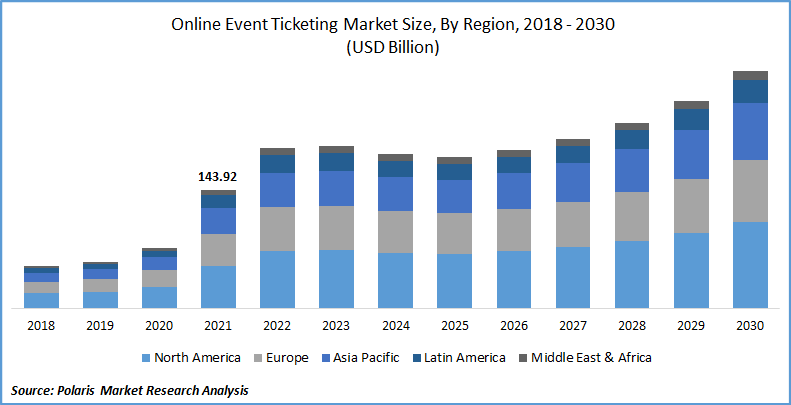
\includegraphics[width=\textwidth]{\FIGDIR/polaris-market-research}
    \source[\citeauthor{online_ticketing_polaris_market_research}]{}
    \label{fig:polaris-market-research}
\end{figure}

Avšak s rapidním vývojem v oblasti webových technologií je důležité sledovat a využívat nové trendy a technologie a přizpůsobovat jim takováto řešení, aby byla pro zákazníky stále atraktivní a relevantní.
Tato práce se proto zaměřuje na vývoj frontendové části webové aplikace prodeje vstupenek s rezervací míst, která bude využívat moderní webové technologie a nástroje, které jsou v současné době nejvíce využívané a oblíbené.
\pagebreak

%%% Sekce - Cíle práce
%%%%% Wording: ✅
%%%%% Styling: ✅
%%%%% References: ✅
%%%%% Grammar: ✅
%%% --------------------------------------------------------------
\section*{Cíle práce}
\addcontentsline{toc}{section}{Cíle práce}
\label{sec:uvod-cile-prace}
Cílem této práce je vyvinout prototyp responzivní webové aplikace nabízející prodej vstupenek s rezervací míst se zaměřením převážně na vývoj frontendové části.

Výsledkem této práce bude webová aplikace vyvinuta moderními webovými nástroji a technologiemi, která umožní potenciálním zákazníkům zobrazit mapu areálu nějaké akce či kulturní události, vybrat si jedno či více preferovaných míst, přidat si vstupenky do nákupního košíku a vytvořit tak objednávku.
Tato práce se bude zabývat vývojem takového webového řešení, ale pouze z pohledu frontendové části.
Ostatní funkčnosti, jako například backendový systém či administrační řešení, nebudou součástí této práce.

Nejprve bude ale pro vývoj třeba prozkoumat a analyzovat existující řešení prodeje vstupenek s rezervací míst, které jsou v současné době využívány.
Na základě identifikace klíčových částí takovýchto systémů budou následně vytvořeny dílčí uživatelské příběhy aplikace, které budou sloužit jako základ pro návrh uživatelského rozhraní.

Aby byla práce považována za úspěšně dokončenou, musí být splněny následující cíle:

\begin{itemize}
    \item Byly identifikovány klíčové prvky a funkčnosti webových řešení prodeje vstupenek s rezervací míst.
    \item Byl vytvořen návrh uživatelského rozhraní aplikace na základě definovaných uživatelských příběhů.
    \item Byla vyvinuta responzivní webová aplikace prodeje vstupenek s rezervací míst.
    \item Aplikace byla nasazena do produkčního prostředí.
\end{itemize}
